\pdfoutput=1
\documentclass[11pt]{amsart}
\usepackage{amsmath,amssymb,amsthm}
\usepackage[margin=1.2in]{geometry}
\usepackage{booktabs,adjustbox,graphicx,xcolor}
\usepackage[colorlinks=true,linkcolor=blue,citecolor=blue,urlcolor=blue]{hyperref}
\hypersetup{pdfauthor={Bernd Johannes Wuebben},pdftitle={Uniform Hermitian--Einstein spectra with repeated stable factors}}
\setlength{\emergencystretch}{2em}
\newtheorem{theorem}{Theorem}[section]
\newtheorem{proposition}[theorem]{Proposition}
\newtheorem{lemma}[theorem]{Lemma}
\newtheorem{corollary}[theorem]{Corollary}
\theoremstyle{definition}
\newtheorem{definition}[theorem]{Definition}
\newtheorem{example}[theorem]{Example}
\theoremstyle{remark}
\newtheorem{remark}[theorem]{Remark}
\newcommand{\C}{\mathbb C}
\newcommand{\R}{\mathbb R}
\newcommand{\PP}{\mathbb P}
\newcommand{\End}{\operatorname{End}}
\newcommand{\Hom}{\operatorname{Hom}}
\newcommand{\Ext}{\operatorname{Ext}}
\newcommand{\tr}{\operatorname{tr}}
\newcommand{\rk}{\operatorname{rk}}
\newcommand{\id}{\operatorname{id}}
\newcommand{\op}{\mathrm{op}}
\newcommand{\HE}{\mathrm{HE}}
\newcommand{\dbar}{\bar\partial}
\newcommand{\HH}{\mathcal H}
\newcommand{\hh}{\mathfrak h}
\newcommand{\norm}[1]{\left\lVert #1\right\rVert}
\title[HE spectra with repeated stable factors]{Uniform Hermitian--Einstein spectra\\with repeated stable factors}
\author{Bernd Johannes Wuebben}
\subjclass[2020]{53C07 (primary); 32L05, 58J50, 16G20 (secondary)}
\keywords{Hermitian--Einstein metrics, stability walls, Dolbeault spectrum,
quiver representations, repeated stable factors}
\date{October 29, 2026}
\begin{document}
\begin{abstract}
We prove uniform relative asymptotics for all small positive Dolbeault
eigenvalues on trace-free endomorphism-valued zero-forms for
Hermitian--Einstein metrics on simple two-step extensions
near an equal-slope Kähler polarization. The stable factors may occur with
arbitrary fixed multiplicities, with distinct isomorphism types in the two
layers. The finite comparison operator is the commutator Laplacian on the
full complex multiplicity algebra, evaluated at an independently balanced
representative of the extension. Every small eigenvalue has relative error
bounded by a fixed multiple of the total balanced extension energy, and the remaining spectrum
has a uniform positive lower bound. No lower bound on positive eigenvalue
ratios or stability margins is imposed. The main estimate bounds the
curvature residual against every multiplicity projection by its crossing
energy; a degree argument then compares the actual metric with the balanced
metric without inverting a degenerating finite Hessian. A fixed rank-five
bundle on a product of four projective lines exhibits six small modes and
arbitrarily separated positive scales.
\end{abstract}
\maketitle
\section{Introduction}\label{sec:introduction}

Let a holomorphic bundle become strictly semistable as a Kähler polarization
approaches a wall. On the stable side its Hermitian--Einstein metric may
diverge in a fixed holomorphic frame. The limiting polystable bundle has
additional parallel endomorphisms, and these give rise to small eigenvalues
of the endomorphism Dolbeault Laplacian. When a stable factor is repeated,
the corresponding parallel endomorphisms form a matrix algebra. The small
spectrum therefore contains matrix directions that are absent from a
scalar graph model.

We determine the entire small spectrum for simple extensions of two
polystable layers, uniformly as positive spectral scales separate. The
finite operator is specified by the extension class and a quadratic
moment-map equation. The principal analytical issue is to compare this
independently specified balance with the actual Hermitian--Einstein metric.
An ordinary implicit-function estimate for the finite equation would divide
by its smallest positive eigenvalue. Such an estimate is not uniform near
a face of a stability chamber. We instead use curvature identities for
all multiplicity projections and a finite-dimensional degree argument.

\subsection{Geometric data and normalization}
Let $X$ be a compact connected complex manifold of dimension $d$, and let
$\omega_s$, for $s$ in a neighborhood of $0$ in $\R^k$, be a smooth family
of Kähler forms. Put $dV_s=\omega_s^d/d!$ and $V_s=\int_XdV_s$.
Fix pairwise nonisomorphic locally free bundles $F_v$, of ranks $r_v$,
which are stable and have the same slope with respect to $\omega_0$.
The index set is the disjoint union of nonempty sets $I$ and $J$.
Fix positive multiplicities $m_v$ and a simple holomorphic extension
\begin{equation}\label{eq:extension}
0\longrightarrow S=\bigoplus_{i\in I}F_i\otimes\C^{m_i}
\longrightarrow E\longrightarrow
U=\bigoplus_{j\in J}F_j\otimes\C^{m_j}\longrightarrow0.
\end{equation}
Simple means $H^0(X,\End E)=\C\id_E$. Repetitions are allowed within
either layer; the same stable isomorphism type does not occur in both.
At least one $m_v>1$ in the applications of interest.

After shrinking the parameter neighborhood, suppose the factors have
smoothly varying Hermitian--Einstein metrics $h_{v,s}$. This is the usual
local continuation of the stable factor metrics; it can also be taken as
an explicit hypothesis on the chosen family. Fix their scalar
normalizations. Write $i\Lambda_sF_{h_{v,s}}=\kappa_v(s)\id_{F_v}$ and
\begin{equation}\label{eq:kappa}
R_E=\sum_vr_vm_v,\qquad
\kappa_E(s)=\frac{1}{R_E}\sum_vr_vm_v\kappa_v(s),\qquad
b_v(s)=-r_v\bigl(\kappa_v(s)-\kappa_E(s)\bigr).
\end{equation}
Our curvature convention is $c_1(F)=[i\tr F_h/(2\pi)]$; thus
\begin{equation}\label{eq:degree}
\kappa(F)=\frac{2\pi}{\rk(F)V_s}
\int_Xc_1(F)\wedge\frac{\omega_s^{d-1}}{(d-1)!}.
\end{equation}
All slope comparisons have the same sign in this normalization.
The numbers $b_v$ satisfy $\sum_vm_vb_v=0$. They are coefficients in
the dual trace pairing, so their definition already includes the factor
ranks.

Choose fixed bases of $\Ext^1(F_j,F_i)$ and take their current harmonic
representatives $\beta_{ij,a,s}$. If $Z=(Z_{ij,a})$ is an array of
$m_i$ by $m_j$ matrices, set
\begin{equation}\label{eq:harmonic}
N_s(Z)_{ij}=\sum_a\beta_{ij,a,s}\otimes Z_{ij,a},\qquad
\dbar_{s,Z}=\dbar_G+N_s(Z),\qquad G=S\oplus U,
\end{equation}
and define $q_s(Z)=V_s^{-1}\norm{N_s(Z)}_{L^2}^2$ using
$h_{0,s}=\bigoplus_vh_{v,s}\otimes I_{m_v}$. We retain the actual
harmonic Gram matrices. Fixed cohomology coordinates need not be
orthonormal for varying $s$. The extension $E$ has fixed cohomology
matrices $Z^0$ in this notation.

The group $\mathcal G=\prod_v\mathrm{GL}(m_v,\C)$ acts by
$(g\cdot Z)_{ij,a}=g_iZ_{ij,a}g_j^{-1}$; its compact subgroup is
$K=\prod_v\mathrm U(m_v)$. Define the quadratic moment map by
\begin{equation}\label{eq:momentdefinition}
\sum_v\tr\bigl(Y_v\mu_s(Z)_v\bigr)
=\left.\frac{d}{dt}\right|_{t=0}q_s(e^{tY/2}\cdot Z)
\quad(Y_v=Y_v^*).
\end{equation}
In orthonormal arrow coordinates it is the sum of incoming $ZZ^*$ minus
outgoing $Z^*Z$. We call $Z$ \emph{balanced} at $s$ if
$\mu_s(Z)_v=b_v(s)I_{m_v}$. Finite balancing below concerns the orbit
$\mathcal G\cdot Z^0$, independently of the unknown HE metric.

A collection of subspaces $W_v\subset\C^{m_v}$ is a
\emph{subrepresentation} if $Z^0_{ij,a}W_j\subset W_i$ for every arrow.
It is proper and nonzero if it is neither the whole collection nor zero.
The representation is $b(s)$-stable when
\begin{equation}\label{eq:finite-stability}
\sum_vb_v(s)\dim W_v>0
\quad\text{for every proper nonzero subrepresentation }W.
\end{equation}
This is King's positive sign convention. The real-weight balancing theorem
then supplies a balanced $Z\in\mathcal G\cdot Z^0$, unique up to $K$.
The details and sign conversion are given in Section~\ref{sec:extensions}.

\subsection{The finite spectrum and the main theorem}
Consider the full complex vector space
\begin{equation}\label{eq:finite-space}
\HH=\left\{X=(X_v)\in\bigoplus_vM_{m_v}(\C):
\sum_vr_v\tr X_v=0\right\},\qquad
\norm X_r^2=\sum_vr_v\tr(X_v^*X_v).
\end{equation}
Its complex dimension is $N=\sum_vm_v^2-1$. For a balanced $Z$, define
\begin{equation}\label{eq:finite-form}
\mathcal Q_{s,Z}(X)=q_s([X,Z]),\qquad
[X,Z]_{ij,a}=X_iZ_{ij,a}-Z_{ij,a}X_j.
\end{equation}
Let $\nu_1(s)\le\cdots\le\nu_N(s)$ be its eigenvalues relative to
$\|\cdot\|_r^2$.
Simplicity makes these eigenvalues positive. Compact-unitary invariance
makes them independent of the choice of balanced representative.
They are defined from the geometry, extension orbit, and finite balance.

\begin{theorem}\label{thm:main}
Fix the geometric data above. There are a neighborhood $\mathcal U$ of
$0$ and constants $C,\gamma>0$ with the following properties.
For $s\in\mathcal U$, the bundle $E$ is slope-stable with respect to
$\omega_s$ if and only if its multiplicity representation is
$b(s)$-stable. At such a parameter let $Z$ be balanced and put
\begin{equation}\label{eq:sigma}
\sigma(s)=\sum_{i\in I}m_ib_i(s)=q_s(Z)>0.
\end{equation}
Let $h_{\HE,s}$ be the HE metric whose determinant is the product
determinant metric induced by the fixed factor metrics. The ordered
eigenvalues, counted with complex multiplicity, of
$\Delta_s=\dbar_{\End E}^{*,h_{\HE,s}}\dbar_{\End E}$ on
$L^2(X,\End_0E)$ satisfy
\begin{equation}\label{eq:main-spectrum}
\left|\frac{\lambda_j(s)}{\nu_j(s)}-1\right|\le C\sigma(s)
\quad(1\le j\le N),\qquad \lambda_{N+1}(s)\ge\gamma.
\end{equation}
If $h_{\mathrm{bal},s}$ is the pullback of $h_{0,s}$ through a
determinant-one balancing gauge and the harmonic identification of $E$,
then
\begin{equation}\label{eq:main-metric}
e^{-C\sigma(s)}h_{\mathrm{bal},s}\le h_{\HE,s}
\le e^{C\sigma(s)}h_{\mathrm{bal},s}.
\end{equation}
The constants impose no lower bound on a positive stability margin,
$\nu_1$, or any positive ratio $\nu_j/\nu_k$. No estimate of the form
$|s|=O(\sigma(s))$ is required.
\end{theorem}

The harmonic identification in this statement is fixed by removing the
exact part of the extension form, as in Lemma~\ref{lem:algebra}.
Changing the balanced representative by $K$ leaves the pulled-back metric
unchanged; the remaining common scalar is fixed by the determinant.
The constants may depend on the fixed factors, multiplicities, harmonic
spaces, and smooth parameter neighborhood. They are not asserted uniform
under degeneration of this background or growth of the multiplicities.

The theorem controls endomorphism-valued zero-forms. It is not a statement
about all degrees of the Dolbeault complex or the entire Yang--Mills
Hessian. At a nonsplit strictly semistable boundary point the original
bundle need not admit an HE metric. All occurrences of $h_{\HE,s}$ in
the theorem are on the stable side.

The example in Section~\ref{sec:example} is a fixed rank-five bundle on
$(\PP^1)^4$ with one multiplicity-two target and three scalar sources.
For genuine polarizations depending on $t,\delta>0$, it has
\begin{equation}\label{eq:intro-example}
\lambda_1=\frac54t\delta\bigl(1+O(t)+O(\delta)\bigr),\qquad
\lambda_j\asymp t\ (2\le j\le6),\qquad\lambda_7\ge\gamma.
\end{equation}
The constants are uniform for independently small $t$ and $\delta$.
In particular $\delta=e^{-1/t}$ is allowed.

\subsection{Relation to earlier work and proof structure}
The correspondence between stable bundles and HE metrics is due to
Donaldson and Uhlenbeck--Yau; we use the standard formulation and
endomorphism identities in Kobayashi~\cite{kobayashi1987}.
King~\cite{king1994} relates subrepresentation stability to moment-map
balance. Haiden--Katzarkov--Kontsevich--Pandit~\cite[\S5.1,
Theorem~5.1]{hkkp2023} give the real-weight formulation used here,
including positive masses on the multiplicity algebra.

Clarke--Tipler~\cite[Propositions~3.1--3.2]{clarketipler2024}
construct the local elliptic reduction without an abelian restriction;
their local wall theorem assumes abelian graded automorphisms.
Delloque~\cite[Proposition~4.2 and Theorems~4.8--4.9]{delloque2025}
allows nonabelian graded automorphisms and proves continuity and
quantitative convergence of HYM representatives under metric variation.
His Proposition~4.7 obtains a zero of the geometrically deformed moment
map. These results already supply nonabelian local reduction and HYM
existence. They do not identify that zero, with a relative error tending
to zero uniformly near weak directions, with a zero of the independently
specified quadratic moment map. The distinction is essential for
\eqref{eq:main-spectrum}: an additive error that is small compared with
the total extension energy may dominate the least positive eigenvalue.
All Delloque locators refer to the published version, arXiv version~4.

The repeated-factor harmonic quiver also occurs in the flow theory of
Lam~\cite[Theorems~8.2, 8.7 and Proposition~8.9]{lam2026}; the finite
iterated-logarithmic asymptotics are developed in
\cite[Theorem~5.11]{hkkp2023}. Those comparisons concern bounded metric
distance in a flow problem. The present result is stationary and gives
a multiplicative error tending to one. It extends the distinct-factor
spectral theorem of~\cite{wuebben2026uniform}; no result of that paper
is needed as an unproved step in the argument below.

The new estimate is Proposition~\ref{prop:projection}: the reduced
curvature residual, paired with any orthogonal multiplicity projection,
is bounded by total extension energy times the energy crossing that
projection. Theorem~\ref{thm:calibration} uses this estimate on spectral
projections of a Hermitian gauge logarithm to exclude zeros on the
boundary of a small ball. Brouwer degree gives the desired HE correction
without a uniform inverse for the finite Hessian. Harmonicity then makes
the Schur-complement coupling proportional to each vector's own finite
energy, yielding every relative eigenvalue estimate.

\section{Harmonic extensions and finite balance}\label{sec:extensions}

We first identify the algebra that enters the finite model. The use of
the complete algebra, rather than one scalar per stable type, determines
both the number of small eigenvalues and the correct stability condition.

\begin{lemma}\label{lem:algebra}
For the extension \eqref{eq:extension}, harmonic representatives of its
fixed cohomology class give a presentation \eqref{eq:harmonic} for every
small $s$. In this presentation
\begin{equation}\label{eq:centralizer}
H^0(X,\End E)=
\left\{(X_v)\in\bigoplus_vM_{m_v}(\C):
X_iZ^0_{ij,a}=Z^0_{ij,a}X_j\text{ for all }i,j,a\right\}.
\end{equation}
The two algebras are identified by parallel block endomorphisms.
Every holomorphic isomorphism between two harmonic presentations is a
parallel block gauge in $\mathcal G$. In particular simplicity of $E$
is equivalent to the common centralizer being scalar.
\end{lemma}

\begin{proof}
Stable nonisomorphic bundles of a common slope have no nonzero maps
between them, and each has only scalar endomorphisms; see
\cite[Chapter~V, \S7]{kobayashi1987}. Hence
$\Hom(F_v,F_w)=0$ for $v\ne w$ and
$\End(F_v)=\C\id$. These are statements about the fixed holomorphic
bundles and do not change with $s$.

A smooth splitting of \eqref{eq:extension} gives a closed off-diagonal
form $\eta\in\Omega^{0,1}(\Hom(U,S))$. Its harmonic part is
$N_s(Z^0)$, and $\eta-N_s(Z^0)=\dbar C_s$ for a smooth section
$C_s$ of $\Hom(U,S)$. An upper-triangular unipotent change of splitting
removes this exact part. Products of two source-to-target blocks vanish,
so there is no nonlinear term in this change. The same observation shows
that $\dbar_{s,Z}^2=0$ for every coefficient array $Z$. Taking $C_s$
orthogonal to the kernel gives a smooth choice in $s$. This gauge has
determinant one.

Apply $\Hom(F_i,-)$ to \eqref{eq:extension}. Since
$\Hom(F_i,U)=0$, one obtains
$\Hom(F_i,E)=\Hom(F_i,S)=\C^{m_i}$. The evaluation image
\[
\operatorname{im}\left(\bigoplus_{i\in I}
F_i\otimes\Hom(F_i,E)\longrightarrow E\right)=S
\]
is the displayed locally free subbundle, fiber by fiber. Every
endomorphism preserves it. In a harmonic splitting an endomorphism
therefore has the form $\left(\begin{smallmatrix}A&C\\0&B\end{smallmatrix}\right)$.
Its diagonal equations make $A$ and $B$ parallel multiplicity blocks.
Its remaining equation is
\begin{equation}\label{eq:exact-harmonic}
\dbar C+N_s(Z^0)B-AN_s(Z^0)=0.
\end{equation}
The last two terms are harmonic, since the multiplicity blocks are
parallel. Exact and harmonic forms are orthogonal, so each term in this
decomposition vanishes. Now $C$ is holomorphic and
$\Hom(U,S)=0$, whence $C=0$. Independence of the cohomology bases gives
\eqref{eq:centralizer}. Conversely those equations plainly define a
holomorphic endomorphism. The same proof for an isomorphism between two
presentations gives the asserted gauge statement.
\end{proof}

The separation of stable types across the layers is natural in this
simple two-step setting. Indeed, for any extension of two polystable
layers of equal slope the map
\[
\Hom(U,S)\longrightarrow\End(E),\qquad f\longmapsto\iota f\pi
\]
is injective and has square-zero image. Simplicity forces this space to
vanish. If a stable type occurred in both layers, it would give a nonzero
map from $U$ to $S$. This observation is specific to two polystable
layers and is not a claim about longer filtrations.

\subsection{The real domain and its dual}
The Hermitian logarithms used for metric corrections form
\begin{equation}\label{eq:realspaces}
\hh=\left\{Y_v=Y_v^*: \sum_vr_v\tr Y_v=0\right\},\qquad
\mathcal W=\left\{T_v=T_v^*: \sum_v\tr T_v=0\right\}.
\end{equation}
They are paired by $\langle Y,T\rangle=\sum_v\tr(Y_vT_v)$.
The positive definite real inner product on $\hh$ is
$\langle X,Y\rangle_r=\sum_vr_v\tr(X_vY_v)$; division of the
$v$-th block of $T$ by $r_v$ identifies $\mathcal W$ with $\hh$.
Both $\mu_s(Z)$ and $b=(b_vI_{m_v})$ lie in $\mathcal W$.
Multiplicities $m_v$ and factor ranks $r_v$ have different roles.

For example, at a fixed parameter orthonormalize the harmonic arrow
basis in the volume-normalized inner product. Then
\begin{equation}\label{eq:momentcomponents}
\mu_i(Z)=\sum_{j,a}Z_{ij,a}Z_{ij,a}^*,\qquad
\mu_j(Z)=-\sum_{i,a}Z_{ij,a}^*Z_{ij,a}.
\end{equation}
The rank weights have not disappeared: they occur in $b_v$ and in the
inner product on the endomorphism algebra. In the original cohomology
coordinates the same equations use the corresponding positive Gram
matrices. Changing arrow basis commutes with $\mathcal G$ and preserves
all subrepresentations.

\begin{proposition}\label{prop:balance}
If the fixed representation $Z^0$ is $b$-stable, its orbit contains a
balanced representative. Under the scalar-centralizer hypothesis this
representative is unique up to $K$. For every such representative
\begin{equation}\label{eq:amplitude}
q_s(Z)=\sum_{i\in I}m_ib_i=\sigma.
\end{equation}
The stable real weights for this fixed representation form an open
polyhedral cone in $\{b:\sum_vm_vb_v=0\}$, possibly with empty
intersection with the accessible parameter image.
\end{proposition}

\begin{proof}
The real-weight finite Kempf--Ness theorem
\cite[\S5.1, Theorem~5.1]{hkkp2023} states that a representation admits
a balanced metric precisely when it is polystable. Its weight convention
is $\theta(W)\le0$; setting $\theta_v=-b_v$ gives
\eqref{eq:finite-stability} and \eqref{eq:momentcomponents}.
The positive masses in the group metric are $r_v$. Equivalently the
central endomorphism parameter of that convention is $-b_v/r_v$.
No second rank factor enters \eqref{eq:finite-stability}.
The theorem allows real weights through its logarithmic determinant
potential; no rational approximation is required. The underlying
integral-character statement is King's
\cite[Propositions~3.1--3.2 and Theorem~6.1]{king1994}.

For clarity, uniqueness here can be checked directly. If two balanced
points differ by $g\in\mathcal G$, polar decomposition and a common
scalar give $g=ke^{Y/2}$, with $k\in K$ and $Y\in\hh$.
Diagonalize $Y$ blockwise and denote its eigenvalues by $y_p$.
Writing $w_{pq}$ for the total squared arrow entries from source
eigenvector $q$ to target eigenvector $p$, the function
\begin{equation}\label{eq:convexpotential}
f(t)=q_s(e^{tY/2}\cdot Z)-t\langle Y,b\rangle
\end{equation}
satisfies
\[
f''(t)=\sum_{p,q}(y_p-y_q)^2e^{t(y_p-y_q)}w_{pq}.
\]
For $Y\ne0$ in $\hh$ this is positive: otherwise $Y$ centralizes
$Z$ and must be scalar, contrary to its weighted trace zero.
Balance at both endpoints would give $f'(0)=f'(1)=0$.
Thus $Y=0$. Tracing all target equations in
\eqref{eq:momentcomponents} proves \eqref{eq:amplitude}.
Finally only finitely many dimension vectors $(\dim W_v)$ are
possible, and each gives a linear strict inequality. These define the
claimed cone. The actual polarization image need not fill that cone.
\end{proof}

At balance the sign can also be seen without a stability convention.
If $\Pi_v$ projects onto a subrepresentation, then for each arrow
\[
\tr(\Pi_iZZ^*)-\tr(\Pi_jZ^*Z)
=\|\Pi_iZ(1-\Pi_j)\|_F^2-\|(1-\Pi_i)Z\Pi_j\|_F^2.
\]
The second term is zero. Equality after summation would make both
the subrepresentation and its orthogonal complement invariant; its
projection would then be a nonscalar centralizer element. Thus balance
with scalar centralizer implies precisely the strict positive sign.

A common complex scalar can normalize the bundle determinant of any
balancing gauge to one, since it acts trivially on the arrows and its
bundle determinant is its $R_E$-th power. Choices of scalar phase do
not affect the metric. Together with the unipotent identification in
Lemma~\ref{lem:algebra}, this defines the determinant convention in
Theorem~\ref{thm:main}.

\section{Projected curvature and multiplicity projections}\label{sec:curvature}

All estimates in this section hold on the product of a fixed small
parameter neighborhood and a fixed small ball of coefficient arrays.
The constants are independent of any positive finite eigenvalue.
For each $s$ consider pointwise trace-free, $h_{0,s}$-Hermitian
endomorphisms of $G$. Let $P_s$ be their $L^2$ projection onto the
entire parallel algebra $\hh$, and put $Q_s=1-P_s$.
For $u\in Q_s$ define
\begin{equation}\label{eq:conjugatedcurvature}
\widehat K(s,Z,u)=e^{u/2}
\bigl(i\Lambda_sF_{\dbar_{s,Z},h_{0,s}e^u}\bigr)e^{-u/2}
-\kappa_E(s)I.
\end{equation}
This is Hermitian for $h_{0,s}$. Its pointwise trace vanishes:
the determinant holomorphic structure is the split determinant and
$\tr u=0$, so the determinant curvature is unchanged and has constant
contraction $R_E\kappa_E$.

\begin{lemma}\label{lem:complement}
The equation $Q_s\widehat K(s,Z,u)=0$ has a unique small solution
$u(s,Z)\in Q_s$, smooth in the finite parameters. For every fixed
nonnegative integer $a$,
\begin{equation}\label{eq:uquadratic}
\norm{u(s,Z)}_{C^a}\le C_aq_s(Z).
\end{equation}
It satisfies $u(s,k\cdot Z)=ku(s,Z)k^{-1}$ for $k\in K$.
\end{lemma}

\begin{proof}
At $Z=u=0$ the linearization of \eqref{eq:conjugatedcurvature} in
the real Hermitian metric variable is
\begin{equation}\label{eq:linearization}
L_s=\tfrac12(\Delta_{\dbar,s}+\Delta_{\partial,s}).
\end{equation}
The conjugation in \eqref{eq:conjugatedcurvature} is included in
this formula; it gives the symmetric real linearization even when
the split summands have different mean curvatures. The Kähler
identities give \eqref{eq:linearization}, and
\[
\langle u,L_su\rangle_{L^2}
=\tfrac12\bigl(\|\dbar u\|_{L^2}^2+\|\partial u\|_{L^2}^2\bigr).
\]
Its kernel is the parallel algebra. At $s=0$ this follows from
stability and vanishing cross-Hom groups. For nearby $s$, a zero
of the displayed sum is parallel for the same split connection;
there are no additional parallel maps. Conversely every
multiplicity block is parallel. The positive spectral gap of
$L_0$ on the complement therefore persists uniformly in a small
neighborhood, and so does its elliptic inverse.

Take an integer $\ell>d$, so that the relevant Sobolev spaces are
algebras on the real $2d$-dimensional manifold. The projected equation
is a smooth map from $Q_sH^{\ell+2}$ to $Q_sH^\ell$.
Identify these varying spaces smoothly with those at zero. The
parameter-dependent implicit-function theorem applies because the
derivative $Q_sL_sQ_s$ is uniformly invertible. At $Z=0$, the split
curvature is parallel; hence $u(s,0)=0$.

The first derivative of the contracted curvature in $Z$ vanishes.
Indeed its off-diagonal linear terms are contractions of covariant
derivatives of the harmonic forms $\beta_{ij,a,s}$; the Kähler
identities identify them with their vanishing Dolbeault adjoints.
Thus $D_Zu(s,0)=0$. Taylor expansion gives the quadratic bound in
Sobolev norm. Elliptic regularity gives \eqref{eq:uquadratic} for
each fixed spatial order. The group $K$ preserves the equation,
the entire parallel algebra, and its orthogonal complement.
Uniqueness proves the equivariance. It is unnecessary, and generally
false, that $K$ fix every vector of the parallel algebra.
\end{proof}

Write $\mathcal F_v(s,Z)$ for the volume-normalized integral of the
partial trace over $F_v$ of the $v,v$ block of
$\widehat K(s,Z,u(s,Z))$. Then
\begin{equation}\label{eq:reducedprojection}
\bigl(P_s\widehat K\bigr)_v
=I_{F_v}\otimes\frac{\mathcal F_v(s,Z)}{r_v}.
\end{equation}
In particular $\mathcal F\in\mathcal W$, and the full HE equation
is equivalent to $\mathcal F=0$ once the complement is solved.

\begin{proposition}\label{prop:projection}
There is a smooth residual $\mathcal R(s,Z)\in\mathcal W$ such that
\begin{equation}\label{eq:reducedexpansion}
\mathcal F(s,Z)=-b(s)+\mu_s(Z)+\mathcal R(s,Z),\qquad
\|D_Z^2\mathcal R(s,Z)\|\le Cq_s(Z).
\end{equation}
For every tuple $\Pi=(\Pi_v)$ of orthogonal multiplicity projections,
\begin{equation}\label{eq:projectionestimate}
\left|\sum_v\tr\bigl(\Pi_v\mathcal R_v(s,Z)\bigr)\right|
\le Cq_s(Z)q_s([\Pi,Z]).
\end{equation}
One constant works for all projections and all sufficiently small
$(s,Z)$, including projections of different ranks at different vertices.
\end{proposition}

The last factor measures the squared norm of precisely those arrow
blocks crossing between $\operatorname{im}\Pi$ and its orthogonal
complement. This factor, rather than a norm of $\Pi$ alone, will
retain control at an arbitrarily weak finite direction.

\begin{proof}
At $Z=0$, \eqref{eq:reducedprojection} gives $\mathcal F=-b$.
Harmonicity kills the linear term, as in Lemma~\ref{lem:complement}.
The direct quadratic term in the Chern curvature is the incoming-minus-
outgoing expression \eqref{eq:momentcomponents}, with its current
harmonic Gram form. The quadratic metric correction contributes
$L_su_2$, where $u_2$ is the quadratic Taylor term of $u$. Its
pairing with every parallel block vanishes, because $L_s$ is
self-adjoint and annihilates those blocks. This proves the constant,
linear, and quadratic parts of \eqref{eq:reducedexpansion}.

The unitary which equals $-I$ at all targets and $I$ at all sources
sends $Z$ to $-Z$ and acts trivially by conjugation on the parallel
algebra. Equivariance yields $\mathcal F(s,-Z)=\mathcal F(s,Z)$.
Consequently the cubic term also vanishes. Joint Taylor expansion,
with the background parameter restricted to a relatively compact
neighborhood, gives the Hessian bound in \eqref{eq:reducedexpansion}.
In particular it holds for each nearby $s$, with no comparison
between $|s|$ and $q_s(Z)$.

Fix $\Pi$ and decompose each arrow into its preserving and crossing
parts, writing $Z=A+C$. Explicitly,
\[
A_{ij,a}=\Pi_iZ_{ij,a}\Pi_j+(1-\Pi_i)Z_{ij,a}(1-\Pi_j),
\quad C=Z-A.
\]
The two parts are orthogonal in the harmonic Gram norm, and
$q_s(C)=q_s([\Pi,Z])$. This remains true for nondiagonal arrow
Gram matrices, since preserving and crossing matrix blocks are
orthogonal for each pair of arrow indices.

At $C=0$ the harmonic bundle is a holomorphic direct sum
$G_\Pi\oplus G_{1-\Pi}$. A circle acting scalarly on $G_\Pi$
and trivially on its complement fixes $A$. Equivariance and
uniqueness of $u$ force $u(s,A)$ to preserve this sum. Integrated
Chern--Weil trace on the first summand is its degree, whence
\begin{equation}\label{eq:projectiondegree}
\sum_v\tr(\Pi_v\mathcal F_v(s,A))
=\sum_vr_v\rk(\Pi_v)(\kappa_v-\kappa_E)
=-\sum_v\tr(\Pi_vb_vI).
\end{equation}
Conjugation by $e^{u/2}$ does not change this trace because it
preserves the summand. The moment-map trace on that summand is
zero: every remaining arrow begins and ends within the same
summand. Thus $\langle\Pi,\mathcal R(s,A)\rangle=0$.

The unitary $2\Pi-I$ fixes $A$ and reverses $C$. It commutes with
$\Pi$, so $\langle\Pi,\mathcal R(s,A+C)\rangle$ is even in $C$.
Its first derivative at $C=0$ vanishes. Taylor expansion in $C$
alone, and the Hessian bound along $A+tC$, now give
\[
|\langle\Pi,\mathcal R(s,A+C)\rangle|
\le Cq_s(A+C)q_s(C).
\]
Here $q_s(A+tC)\le q_s(A+C)$ for $0\le t\le1$ by orthogonality.
The finitely many rank choices of $\Pi$ give compact products of
Grassmannians; unitary invariance and bounded derivatives make
the constant independent of $\Pi$. This proves
\eqref{eq:projectionestimate}.
\end{proof}

Only the auxiliary representation $A$, with its crossing blocks removed,
was used to form the holomorphic direct summand in the proof.
The projection $\Pi$ need not define a holomorphic subbundle for the
original representation $Z$. This is why
\eqref{eq:projectionestimate} is available for every orthogonal
projection, including the spectral projections used next.

\section{Comparison with an independently balanced metric}\label{sec:calibration}

The reduced finite equation differs from quadratic balance by the
residual of Proposition~\ref{prop:projection}. Its derivative may have
arbitrarily small positive eigenvalues. We obtain the required metric
correction by excluding zeros on the boundary of a small ball, rather
than estimating the inverse of that derivative.

\begin{theorem}\label{thm:calibration}
There are constants $A,\sigma_0>0$ such that the following holds
uniformly in the fixed background neighborhood. Let $Z$ satisfy
$\mu_s(Z)=b(s)$, let its complex centralizer be scalar, and suppose
$0<\sigma=q_s(Z)<\sigma_0$. Then some $Y\in\hh$ satisfies
\begin{equation}\label{eq:calibration}
\|Y\|_{\op}\le A\sigma,\qquad
\mathcal F(s,e^{Y/2}\cdot Z)=0.
\end{equation}
For $Z'=e^{Y/2}\cdot Z$, the metric $h_{0,s}e^{u(s,Z')}$ is HE
on $E_{s,Z'}$, and $\|u(s,Z')\|_{C^a}\le C_a\sigma$ for every
fixed $a$. The constants do not depend on a positive finite
eigenvalue or on a ratio of such eigenvalues.
\end{theorem}

\begin{proof}
On the real space $\hh$ consider the homotopy into $\mathcal W$
\begin{equation}\label{eq:homotopy}
H_\tau(Y)=\mu_s(e^{Y/2}\cdot Z)-b+
\tau\mathcal R(s,e^{Y/2}\cdot Z),\qquad 0\le\tau\le1.
\end{equation}
Use the ball $\|Y\|_{\op}<a$, where $a=A\sigma<1$ and
$\|Y\|_{\op}=\max_v\|Y_v\|_{\op}$. Write
$M=\sum_vm_v$. Both layers are nonzero, so $M\ge2$.

Suppose $\|Y\|_{\op}=a$. Diagonalize each block of $Y$ unitarily
and sort all $M$ eigenvalues as $y_1\le\cdots\le y_M$, retaining
their vertices. The condition $\sum_vr_v\tr Y_v=0$, with positive
weights, implies that their oscillation is at least $a$. An adjacent
gap therefore satisfies
\begin{equation}\label{eq:gapchoice}
\delta=y_{\ell+1}-y_\ell\ge\frac{a}{M-1}.
\end{equation}
Let $\Pi$ be the tuple of spectral projections onto eigenvectors
above this gap. It is nonzero and proper and commutes with $Y$.

Use orthonormal arrow coordinates at this fixed $s$. If $p$ is a
target eigenvector and $q$ a source eigenvector, write $w_{pq}$ for
the sum of squared arrow entries joining them. The gauge
$e^{Y/2}$ multiplies $w_{pq}$ by $e^{y_p-y_q}$. Since $\mu_s(Z)=b$,
\begin{align}
\langle\Pi,\mu_s(e^{Y/2}\cdot Z)-b\rangle
&=\sum_{p,q}(\Pi_p-\Pi_q)(e^{y_p-y_q}-1)w_{pq}\notag\\
&\ge(1-e^{-\delta})q_s([\Pi,Z])\notag\\
&\ge e^{-2a}\frac{a}{M-1}q_s([\Pi,Z]).\label{eq:boundarypositive}
\end{align}
For a high target and low source the exponential difference is
positive and at least $e^\delta-1$. For a low target and high
source the projection sign is negative and its product with the
exponential difference is at least $1-e^{-\delta}$. These are all
crossing entries; preserving entries contribute zero. The last
inequality follows from $\delta\le2a$ and
$1-e^{-\delta}\ge\delta e^{-\delta}$.
The crossing energy is strictly positive. Otherwise $\Pi$ would
commute with every arrow and be a nonscalar centralizer element.

Put $Z_Y=e^{Y/2}\cdot Z$. The gauge bounds and $[\Pi,Y]=0$ give
\begin{equation}\label{eq:crossingbounds}
q_s(Z_Y)\le e^{2a}\sigma,\qquad
q_s([\Pi,Z_Y])\le e^{2a}q_s([\Pi,Z]).
\end{equation}
Proposition~\ref{prop:projection} consequently yields
\begin{equation}\label{eq:boundaryerror}
|\langle\Pi,\mathcal R(s,Z_Y)\rangle|
\le Ce^{4a}\sigma q_s([\Pi,Z]).
\end{equation}
Choose $A>2C(M-1)$, and then choose $\sigma_0$ so small that
$e^{6A\sigma_0}<2$ and the entire gauge ball stays in the
coefficient neighborhood. Since $a=A\sigma$,
\eqref{eq:boundarypositive} strictly dominates
\eqref{eq:boundaryerror}. Thus $H_\tau$ has no zero on the
boundary, for any $\tau\in[0,1]$. The projection depends on $Y$;
only pointwise exclusion of a boundary zero is needed.

At $\tau=0$ the unique zero is $Y=0$. Indeed the function
\eqref{eq:convexpotential} has $f'(0)=0$ and $f''(t)>0$ for
nonzero $Y\in\hh$, by the scalar-centralizer hypothesis.
It follows that $\langle Y,H_0(Y)\rangle=f'(1)>0$.
The derivative at zero also satisfies
\begin{equation}\label{eq:finitehessian}
\langle Y,DH_0(0)Y\rangle=q_s([Y,Z])>0\quad(Y\ne0).
\end{equation}
Under the fixed identification $T_v\mapsto T_v/r_v$ from
$\mathcal W$ to $\hh$, this is a positive definite real Hessian.
Its local Brouwer degree is $+1$. The operator-norm ball is a
bounded open subset of a finite-dimensional real vector space;
smoothness of its boundary is not required for degree. Homotopy
invariance gives a zero of $H_1$ inside this ball.

At that zero the reduced equation and the complementary equation
both vanish, so \eqref{eq:conjugatedcurvature} is zero. This is
the HE equation. Finally \eqref{eq:crossingbounds} and
Lemma~\ref{lem:complement} give the asserted bounds for $u$.
\end{proof}

The positivity in \eqref{eq:finitehessian} is used to compute a
degree at each fixed parameter. No uniform lower bound for this
Hessian is used. Likewise the crossing energy in
\eqref{eq:boundarypositive} may be arbitrarily small; it appears
as the same positive factor in the error bound and cancels in the
comparison. This gives the uniformity at weak directions.

\begin{proposition}\label{prop:actual-stability}
After shrinking the parameter neighborhood, $E$ is slope-stable
exactly at the $b(s)$-stable points of its representation.
At these points the metric comparison \eqref{eq:main-metric} holds.
\end{proposition}

\begin{proof}
Let $W$ be a proper nonzero subrepresentation. The smooth subbundle
$G_W=\bigoplus_vF_v\otimes W_v$ is preserved by
$\dbar_{s,Z^0}$ and hence is an actual holomorphic subbundle of $E$
with locally free quotient. Put $r_W=\sum_vr_v\dim W_v$.
Its degree is the sum of the degrees of its factor copies, so
\begin{equation}\label{eq:subbundle-slope}
\kappa(G_W)-\kappa_E
=-\frac{\sum_vb_v\dim W_v}{r_W}.
\end{equation}
Stability of $E$ forces the inequalities
\eqref{eq:finite-stability}. This implication uses only the
displayed subbundles, without asserting that they exhaust all
subsheaves.

Conversely, finite stability gives a balanced $Z$ by
Proposition~\ref{prop:balance}. Lemma~\ref{lem:algebra} gives
its scalar centralizer. Since $b(0)=0$, shrink the background
neighborhood so that every such $\sigma$ is below the fixed
threshold of Theorem~\ref{thm:calibration}. That theorem constructs
an HE metric on $E_{s,Z'}$, and the harmonic and finite gauges pull
it back to $E$. An HE bundle is polystable
\cite[Chapter~V]{kobayashi1987}; a simple polystable bundle has
only one stable summand, and therefore is stable. This argument
constructs the HE metric before using stability sufficiency.

For the comparison, work first on the independently balanced
presentation. With $g=e^{Y/2}$ the additional pullback of the
metric has matrix $g^*e^ug$ in a split unitary frame. Scalar
Hermitian-form bounds for $e^u$ and for $g^*g=e^Y$ give
\[
e^{-C\sigma}h_{0,s}\le g^*(h_{0,s}e^u)
\le e^{C\sigma}h_{0,s}.
\]
No commutation of $u$ and $Y$ is needed. Pullback through the
same original balancing gauge and harmonic identification
preserves these inequalities, even if the balancing gauge is
unbounded. This proves \eqref{eq:main-metric}. The unipotent
identification and determinant-normalized finite gauges have
determinant one; $\sum_vr_v\tr Y_v=0$ and $\tr u=0$ preserve
the fixed determinant metric. The HE metric is unique after
this normalization.
\end{proof}

No smooth selection of $Y$ as the parameter approaches a chamber
face is asserted. The proof supplies a uniformly small correction
at every stable point. Bounds for derivatives of a selected gauge
with respect to the parameter are a different question.

\section{The full small Dolbeault spectrum}\label{sec:spectrum}

We now compare the elliptic operator with the finite form. The first
step holds for every sufficiently small simple coefficient array,
whether balanced or not. All Hilbert spaces in this section are
complex, and all endomorphisms are pointwise trace-free.

\begin{proposition}\label{prop:schur}
Let $Z'$ be small with scalar centralizer. Use the split metric
$h_{0,s}$ on $E_{s,Z'}$, and let $\nu_j(s,Z')$ be the eigenvalues
of \eqref{eq:finite-form}. There are constants $C,\gamma_1>0$,
uniform in the fixed background neighborhood, such that the
ordered Dolbeault eigenvalues $\widetilde\lambda_j$ satisfy
\begin{equation}\label{eq:schurbound}
(1-Cq_s(Z'))\nu_j(s,Z')\le\widetilde\lambda_j
\le\nu_j(s,Z')\quad(1\le j\le N),\qquad
\widetilde\lambda_{N+1}\ge\gamma_1/2.
\end{equation}
In particular exactly $N$ eigenvalues lie below a fixed positive
threshold for sufficiently small $Z'$.
\end{proposition}

\begin{proof}
Write $D_0=\dbar_{\End G}$ and
$D=D_0+\mathcal A$, where $\mathcal A=[N_s(Z'),\,\cdot\,]$.
The kernel of $D_0$ is the full parallel space $\HH$ of
\eqref{eq:finite-space}, by the fixed cross-Hom vanishing.
Let $P$ be complex $L^2$ projection onto $\HH$, and put $Q=1-P$.
These are the complex spectral projections, distinct from the
real metric-coordinate projections of Section~\ref{sec:curvature}.
The positive spectrum of $D_0^*D_0$ on $Q$ has a uniform lower
bound $\gamma_0>0$.

For every parallel $X\in\HH$, $\mathcal AX$ is harmonic,
because it is a constant multiplicity combination of the harmonic
Hom forms. Thus
\begin{equation}\label{eq:harmoniccancel}
D_0^*\mathcal AX=0,\qquad
V_s^{-1}\|DX\|_{L^2}^2=\mathcal Q_{s,Z'}(X),\qquad
V_s^{-1}\|X\|_{L^2}^2=\|X\|_r^2.
\end{equation}
Let $q=q_s(Z')$. Since the harmonic coefficient space is fixed and
finite-dimensional, its $C^0$ and $L^2$ norms are uniformly
equivalent. Consequently
$\|\mathcal A\|_{L^2\to L^2(0,1)}\le C\sqrt q$.
For $y\in QH^1$ this gives
\[
\|Dy\|_{L^2}\ge(\sqrt{\gamma_0}-C\sqrt q)\|y\|_{L^2}.
\]
The complementary compression $C_0=QD^*DQ$, understood initially
as a closed quadratic form, therefore satisfies $C_0\ge\gamma_1I$
for some fixed $\gamma_1>0$ and all sufficiently small $q$.

Set $G_0=PD^*DP$ and $B=QD^*DP$. Harmonicity in
\eqref{eq:harmoniccancel} gives, as equalities of smooth sections,
\begin{equation}\label{eq:relativecoupling}
BX=Q\mathcal A^*\mathcal AX,\qquad
\|BX\|_{L^2}^2\le Cq\|\mathcal AX\|_{L^2}^2
=Cq\langle X,G_0X\rangle_{L^2}.
\end{equation}
The right side is each vector's own finite energy. There is no
replacement by $q\|X\|^2$ and no division by $\nu_1$.

We specify the form domains to justify the spectral comparison.
The form domain of $D^*D$ is $H^1(\End_0G)$ and its operator
domain is $H^2(\End_0G)$. Removing the finite-dimensional smooth
space $\HH$ preserves these Sobolev spaces; the form and operator
domains of $C_0$ are $QH^1$ and $QH^2$. In particular $B$ maps
the finite space into $L^2$, and $(C_0-\lambda)^{-1}$ maps $QL^2$
into $QH^2$ for $0\le\lambda\le\gamma_1/2$.

For such $\lambda$ define the finite Schur complement
\begin{equation}\label{eq:schur}
S_\lambda=G_0-\lambda I-B^*(C_0-\lambda)^{-1}B.
\end{equation}
Equation~\eqref{eq:relativecoupling} gives the Hermitian-form bounds
\begin{equation}\label{eq:schurforms}
(1-Cq)G_0-\lambda I\le S_\lambda\le G_0-\lambda I.
\end{equation}
Completion of the square on $\HH\oplus QH^1$ gives
\begin{align}
\mathfrak q_{D^*D-\lambda}(X+y)
={}&\langle S_\lambda X,X\rangle\notag\\
&+\left\|(C_0-\lambda)^{1/2}
\bigl(y+(C_0-\lambda)^{-1}BX\bigr)\right\|^2.\label{eq:inertia}
\end{align}
The triangular change of variables here is a bijection of the
form domain, since its correction lies in $QH^2$. The negative
index of $D^*D-\lambda$ thus equals the negative index of
$S_\lambda$.

The norm of $G_0$ is $O(q)$. At $\lambda=\gamma_1/2$ the
finite Schur complement is strictly negative, whereas the
complementary operator is positive. Exactly $N$ eigenvalues
therefore lie below this threshold and the threshold is not an
eigenvalue. For the indexed lower bound put $\alpha=1-Cq>0$.
If $\lambda<\alpha\nu_j$, the form $\alpha G_0-\lambda I$
has at most $j-1$ negative directions. The same is true of
$S_\lambda$ by \eqref{eq:schurforms}; \eqref{eq:inertia}
then implies $\widetilde\lambda_j\ge\alpha\nu_j$ by passage
to the limit. For the upper bound apply ordinary min--max to
the first $j$ finite eigenvectors inside $\HH$.
These arguments also apply when eigenvalues coincide. They
establish \eqref{eq:schurbound} with complex multiplicities.
\end{proof}

\begin{lemma}\label{lem:gaugespectrum}
Let $g=e^{Y/2}$ for $Y\in\hh$, put $a=\|Y\|_{\op}$, and let
$Z'=g\cdot Z$. For all $1\le j\le N$,
\begin{equation}\label{eq:gaugecomparison}
e^{-4a}\nu_j(s,Z)\le\nu_j(s,Z')\le e^{4a}\nu_j(s,Z).
\end{equation}
This comparison holds for arbitrary positive harmonic Gram matrices.
\end{lemma}

\begin{proof}
Conjugation $T_gX=(g_vX_vg_v^{-1})_v$ preserves the full complex
space $\HH$, since it preserves each block trace. The bounds
$\|g_v^{\pm1}\|_{\op}\le e^{a/2}$ imply
\begin{equation}\label{eq:gaugemass}
e^{-2a}\|X\|_r^2\le\|T_gX\|_r^2\le e^{2a}\|X\|_r^2.
\end{equation}
The exact intertwining identity
\[
[T_gX,g\cdot Z]_{ij,a}=g_i[X,Z]_{ij,a}g_j^{-1}
\]
gives the same factors for the squared energy. For a nondiagonal
Gram matrix, apply its positive square root to the arrow index.
Left and right multiplicity operations commute with this change
because every arrow in the block has the same source and target.
Thus the same energy bounds hold without changing constants.
Rayleigh quotients have factors $e^{\pm4a}$, and generalized
min--max through the invertible complex map $T_g$ proves the lemma.
\end{proof}

The map $T_g$ need not preserve Hermitian matrices. Its use on
$\HH$ is one reason to retain the full complex operator throughout
the argument. At exact central balance there is an additional
adjoint symmetry, discussed in Section~\ref{sec:scope}, but no
such symmetry is needed during this comparison.

\begin{proof}[Proof of Theorem~\ref{thm:main}]
Proposition~\ref{prop:actual-stability} proves the stability
equivalence and metric statement. At a stable parameter choose
the independently balanced $Z$. Theorem~\ref{thm:calibration}
gives $Z'=e^{Y/2}\cdot Z$ with $\|Y\|_{\op}\le A\sigma$
and $\|u\|_{C^0}\le C\sigma$. Moreover
$q_s(Z')\le e^{2A\sigma}\sigma$.
Proposition~\ref{prop:schur} and Lemma~\ref{lem:gaugespectrum}
therefore compare the split-metric small eigenvalues at $Z'$
to $\nu_j(s,Z)$ with a common factor $1+O(\sigma)$.

It remains to pass to the actual metric on the same holomorphic
bundle $E_{s,Z'}$. If two bundle metrics satisfy
$e^{-c}h_0\le h_1\le e^ch_0$, their induced squared norms on
$\End G$ lie between $e^{-2c}$ and $e^{2c}$ times each other.
The same is true on $\End G$-valued $(0,1)$-forms, since the
base metric is fixed in this comparison. The differential $D$
is unchanged. Hence every Rayleigh quotient has comparison
factors $e^{\pm4c}$ on the common $H^1$ form domain. Apply this
with $h_1=h_{0,s}e^u$ and $c=C\sigma$.

The trace-free spaces in this argument are invariant for both
Laplacians. Indeed $\End G=\C I\oplus\End_0G$ is orthogonal
for every induced endomorphism metric, $D(fI)=(\dbar f)I$, and
$\tr(D\xi)=\dbar\tr\xi$. This orthogonal splitting also
holds on one-forms. Both $D$ and its adjoint preserve the
corresponding summands. Min--max therefore applies to the same
trace-free domain for each metric.

The additional factor is $1+O(\sigma)$, so it proves
\eqref{eq:main-spectrum} for $1\le j\le N$. It also leaves a
fixed positive fraction of the complementary bound in
Proposition~\ref{prop:schur}. Finally holomorphic pullback,
with the metric pulled back at the same time, is unitary on
the relevant $L^2$ spaces and intertwines the Dolbeault
operators. It identifies these eigenvalues with those on
the original $E$, regardless of the size of the original
balancing gauge. Shrinking $\mathcal U$ absorbs all uniform
exponential factors into the stated constants.
\end{proof}

\section{A fixed rank-five bundle with separated spectral scales}\label{sec:example}

We give a geometric example in which the stable region has three
independent polarization parameters. Its full finite model has six
complex modes, and one can tend to zero at an arbitrary positive
rate relative to the other five.

Let $X=(\PP^1)^4$. Write $\omega_\ell$ for the pullbacks of
Fubini--Study forms normalized by $\int_{\PP^1}\omega_\ell=1$,
and put $\omega_h=\sum_{\ell=1}^4h_\ell\omega_\ell$, with
$h_\ell>0$. Consider
\begin{equation}\label{eq:linebundles}
F_0=\mathcal O_X,\qquad F_j=\mathcal O_X(2e_j-2e_4)\quad(1\le j\le3),
\end{equation}
where $e_\ell$ denotes degree one on the $\ell$-th factor, and
an extension
\begin{equation}\label{eq:star-extension}
0\longrightarrow\mathcal O_X\otimes\C^2\longrightarrow E
\longrightarrow F_1\oplus F_2\oplus F_3\longrightarrow0.
\end{equation}
All four stable types are line bundles. They are distinct and have
degree zero at $h=(1,1,1,1)$. Product invariant Hermitian metrics are
HE for every product polarization. The normalization
\eqref{eq:degree} gives
\begin{equation}\label{eq:linecurvature}
V_h=h_1h_2h_3h_4,\qquad\kappa_0=0,\qquad
\kappa_j=4\pi(h_j^{-1}-h_4^{-1}),\qquad
\kappa_E=\tfrac15\sum_{j=1}^3\kappa_j.
\end{equation}
Indeed $iF_{F_j}=4\pi(\omega_j-\omega_4)$ and
$\Lambda_{\omega_h}\omega_\ell=h_\ell^{-1}$.

The Künneth formula and line-bundle cohomology on $\PP^1$ give
\begin{equation}\label{eq:extstar}
\Ext^1(F_j,F_0)=
H^1(\PP^1,\mathcal O(-2))\otimes H^0(\PP^1,\mathcal O(2))
\cong\C^3.
\end{equation}
The nonconstant factors are $j$ and $4$; the others contribute
$H^0(\mathcal O)=\C$. Fix cohomology bases orthonormal at the
reference polarization in the volume-normalized inner product.
For every $h$, the current harmonic Gram matrix is $c_j(h)I_3$
with $c_j(h)>0$ smooth. To see this, all the chosen metrics and
forms are invariant under $\mathrm{SU}(2)^4$. The only nontrivial
action on \eqref{eq:extstar} is the irreducible three-dimensional
representation on the fourth-factor degree-two sections.
Schur's lemma makes the invariant harmonic inner product a scalar
multiple of the reference one. The cohomology coefficients below
remain fixed as the harmonic representatives vary.

For small real $a=(a_1,a_2,a_3)$ let $A=a_1+a_2+a_3$ and choose
the actual polarization chart
\begin{equation}\label{eq:chart}
h_4=1,\qquad
h_j=\left(1+\frac{A/2+a_j}{4\pi}\right)^{-1}\quad(1\le j\le3).
\end{equation}
It is defined for all sufficiently small signed $a$ and has
positive coefficients. Substitution into \eqref{eq:linecurvature}
gives
\begin{equation}\label{eq:demands}
\kappa_E=A/2,\qquad\kappa_j-\kappa_E=a_j,\qquad
b_0=A/2,\qquad b_j=-a_j,\qquad\sigma=A.
\end{equation}
The target moment is $(A/2)I_2$, so its trace is $A$. Thus the
three finite demands are independent geometric parameters.

\subsection{The extension and its complete endomorphism algebra}
Define the fixed extension class by the following matrices, whose
three columns multiply the basis elements in \eqref{eq:extstar}:
\begin{equation}\label{eq:Zstar}
\begin{split}
Z_1^0&=\begin{pmatrix}\sqrt{3/2}&0&0\\0&1/\sqrt2&0\end{pmatrix},\qquad
Z_2^0=\begin{pmatrix}1&0&0\\1/2&\sqrt3/2&0\end{pmatrix},\\
Z_3^0&=\begin{pmatrix}1/\sqrt2&0&0\\-1/\sqrt2&1&0\end{pmatrix}.
\end{split}
\end{equation}
An extension of locally free sheaves by locally free sheaves is
locally free. These classes therefore define one fixed rank-five
holomorphic bundle, rather than merely a finite representation.
The covariances $B_j=Z_j^0(Z_j^0)^*$ are
\begin{equation}\label{eq:Bstar}
B_1=\begin{pmatrix}3/2&0\\0&1/2\end{pmatrix},\quad
B_2=\begin{pmatrix}1&1/2\\1/2&1\end{pmatrix},\quad
B_3=\begin{pmatrix}1/2&-1/2\\-1/2&3/2\end{pmatrix}.
\end{equation}
They have determinants $3/4,3/4,1/2$, respectively, and
\begin{equation}\label{eq:noncommute}
B_1+B_2+B_3=3I_2,\qquad
[B_1,B_2]=\begin{pmatrix}0&1/2\\-1/2&0\end{pmatrix}\ne0.
\end{equation}
In particular the interactions are not simultaneously diagonal.

If $XZ_j^0=Z_j^0x_j$ for $X\in M_2(\C)$ and scalar $x_j$,
full row rank of each $Z_j^0$ implies $X=x_jI_2$.
All $x_j$ coincide. Lemma~\ref{lem:algebra} proves that $E$ is
simple. The full trace-free complex space is
\begin{equation}\label{eq:starspace}
\HH=\{(X,x_1,x_2,x_3):\tr X+x_1+x_2+x_3=0\},\qquad
\|(X,x)\|^2=\|X\|_F^2+\sum_j|x_j|^2.
\end{equation}
It has dimension six. The multiplicity two of the target is
already included in its matrix trace; it is not an additional
factor rank.

\begin{proposition}\label{prop:starbalance}
The local stable region of the fixed bundle \eqref{eq:star-extension}
in the chart \eqref{eq:chart} is exactly $a_1,a_2,a_3>0$.
For these parameters its balanced covariances are
\begin{equation}\label{eq:targetbalance}
C_j=a_j\frac{TB_jT}{\tr(TB_jT)},\qquad
\sum_{j=1}^3C_j=\frac A2I_2,
\end{equation}
where $T$ is positive Hermitian and $\det T=1$.
The target shape $T$ is unique, uniformly bounded together with
its inverse, and smooth in the normalized weights $w_j=a_j/A$
on the entire closed simplex.
\end{proposition}

\begin{proof}
If a subrepresentation contains any source, its target contains
the span of that source's three images, which is all of $\C^2$.
The proper nonzero subrepresentations therefore have either a
target line and no sources, or the full target with a proper
subset $S$ of sources. Their demands are $A/2$ and
$\sum_{j\notin S}a_j$, respectively. They are all positive
when $a_j>0$. Conversely, taking the full target and every
source except $j$ gives demand $a_j$, so finite stability
requires all three to be positive. Theorem~\ref{thm:main}
identifies this with the actual local stable region.

The scalar harmonic Gram factor $c_j(h)$ can be absorbed into
the positive gauge at source $j$. After a target gauge $T$,
choose its source multiplier to have square
$c_j(h)\tr(TB_jT)/a_j$. This produces \eqref{eq:targetbalance}
in the same extension orbit. A common scalar on all blocks
normalizes the entire bundle determinant; $\det T=1$ fixes only
the target shape.

To prove existence and uniformity directly, put $H=T^2$ and
minimize
\begin{equation}\label{eq:targetpotential}
f_w(H)=\sum_jw_j\log\tr(HB_j),\qquad H=H^*>0,\quad\det H=1.
\end{equation}
All $B_j$ are positive definite. With $c=1-1/\sqrt2>0$,
one has $B_j\ge cI$ and $f_w(I)=\log2$. Therefore
\[
f_w(H)\ge\log(c\tr H),\qquad
\tr H\le\frac2c=4+2\sqrt2
\quad\text{at a minimizer}.
\]
This is a uniform coercivity bound for all weights in the
closed simplex. The determinant condition bounds both
eigenvalues above and away from zero on the indicated sublevel
set, proving existence and compactness of the minimizers.

For a determinant-one geodesic
$H(t)=H_0^{1/2}e^{tY}H_0^{1/2}$ with $Y=Y^*$ and $\tr Y=0$,
each summand of \eqref{eq:targetpotential} is
$\log\sum_\ell q_{j\ell}e^{ty_\ell}$ in an eigenbasis for $Y$.
Every $q_{j\ell}$ is strictly positive, because $B_j>0$.
The second derivative is the variance of the $y_\ell$ under
positive normalized weights. It is strictly positive when
$Y\ne0$. A convex combination of these variances remains
positive even if some $w_j=0$. Hence $f_w$ is strictly geodesically
convex and the minimizer is unique.

At $H=T^2$ its first variation in direction $TYT$ is
\[
\tr\left(Y\sum_jw_j\frac{TB_jT}{\tr(TB_jT)}\right).
\]
It vanishes for every trace-free Hermitian $Y$ exactly when the
matrix in parentheses is $I_2/2$, proving
\eqref{eq:targetbalance}. On the compact family of minimizers
the Hessian has a uniform positive lower bound on unit tangent
vectors. The finite-dimensional implicit-function theorem gives
a smooth extension near each point of the closed simplex in its
affine weight hyperplane. Uniqueness patches these extensions.
This proves the asserted smoothness, including at corners.
\end{proof}

At a boundary weight the corresponding limiting arrow disappears.
The source gauge relating it to the original nonzero class is no
longer invertible there. Boundedness of $T$ is not boundedness of
the full metric, and the proposition asserts no HE metric on the
original boundary bundle.

\subsection{Six finite modes}
For the covariances \eqref{eq:targetbalance}, the finite form is
\begin{equation}\label{eq:starform}
\mathcal Q(X,x)=\sum_{j=1}^3
\tr\bigl((X-x_jI)C_j(X-x_jI)^*\bigr)
\quad\text{on \eqref{eq:starspace}}.
\end{equation}
At $a_1=a_2=a_3=2t$ one has $T=I$ and $C_j=tB_j$.

\begin{proposition}\label{prop:sixmodes}
At these equal demands the six finite eigenvalues, divided by $t$,
are
\begin{equation}\label{eq:sixmodes}
3,\quad5,\quad\frac{5-\sqrt7}{2},\quad\frac{5+\sqrt7}{2},\quad
\frac{5-\sqrt3}{2},\quad\frac{5+\sqrt3}{2}.
\end{equation}
The scalar-target compression instead has only three positive
eigenvalues, $2t,2t,5t$.
\end{proposition}

\begin{proof}
It suffices to take $t=1$. In $M_2(\C)$ use the orthonormal basis
\[
I_2/\sqrt2,\qquad\sigma_z/\sqrt2,\qquad
\sigma_x/\sqrt2,\qquad\sigma_y/\sqrt2,
\]
where the last three are the Pauli matrices. Their complex span
is the full matrix algebra. On the complete seven-dimensional
space before removing the identity, \eqref{eq:starform} has matrix
\begin{equation}\label{eq:staroperator}
L=\begin{pmatrix}3I_4&-K\\-K^*&2I_3\end{pmatrix},\qquad
K=\begin{pmatrix}
\sqrt2&\sqrt2&\sqrt2\\
1/\sqrt2&0&-1/\sqrt2\\
0&1/\sqrt2&-1/\sqrt2\\
0&0&0
\end{pmatrix}.
\end{equation}
The eigenvalues of $K^*K$ are $6,3/2,1/2$.
Each squared singular value $s^2$ gives the quadratic factor
$(\lambda-3)(\lambda-2)-s^2$, and the remaining target
direction has eigenvalue $3$. Thus
\[
\det(\lambda I_7-L)=\lambda(\lambda-5)(\lambda-3)
(\lambda^2-5\lambda+9/2)(\lambda^2-5\lambda+11/2).
\]
The zero is exactly the scalar identity. Its orthogonal complement
is \eqref{eq:starspace}, which gives \eqref{eq:sixmodes}.
Restricting the target to its scalar part replaces $K$ by its
first row and gives $\lambda(\lambda-5)(\lambda-2)^2$.
\end{proof}

\subsection{Arbitrary separation on genuine polarizations}
Set $a=(t\delta,t,t)$, with $t,\delta>0$. The target solution
depends only on $w=(\delta,1,1)/(2+\delta)$, so the form
$\mathcal Q/t$ is smooth in $\delta$ down to zero.

\begin{theorem}\label{thm:star-scales}
There are $t_0,\delta_0,c,C,\gamma>0$ such that, for independently
chosen $0<t<t_0$ and $0<\delta<\delta_0$, the HE spectrum of the
fixed bundle \eqref{eq:star-extension} at \eqref{eq:chart} satisfies
\begin{equation}\label{eq:staractual}
\lambda_1=\frac54t\delta\bigl(1+O(\delta)+O(t)\bigr),\qquad
ct\le\lambda_j\le Ct\ (2\le j\le6),\qquad
\lambda_7\ge\gamma.
\end{equation}
All constants are independent of the ratio between $\delta$ and $t$.
\end{theorem}

\begin{proof}
At $\delta=0$ the target and sources $2,3$ form a simple
representation, since each of these sources has full image span.
The absent first source adds one centralizer direction. On
\eqref{eq:starspace} the kernel is therefore exactly the line
\begin{equation}\label{eq:weakkernel}
(X,x_1,x_2,x_3)=(\alpha I_2,-4\alpha,\alpha,\alpha).
\end{equation}
Its squared norm is $20|\alpha|^2$, and the remaining five
eigenvalues of $\mathcal Q/t$ are positive. On this fixed vector
the strong-source terms vanish for every target shape. Since
$\tr C_1=t\delta$, the weak-source term is exactly
$25t\delta|\alpha|^2$. Smooth perturbation of the simple zero
eigenvalue gives
\begin{equation}\label{eq:weakfinite}
\nu_1=\frac54t\delta\bigl(1+O(\delta)\bigr),\qquad
ct\le\nu_j\le Ct\quad(2\le j\le6).
\end{equation}
The derivative $5/4$ is the ratio $25/20$ of energy derivative
to mass. The finite form scales exactly with $t$, so these
constants are uniform in $t>0$.

All $a_j$ are positive, and
$\sigma=t(2+\delta)$. Theorem~\ref{thm:main} applies with
relative error $O(t)$ and a fixed complementary gap. Combining
it with \eqref{eq:weakfinite} proves \eqref{eq:staractual}.
\end{proof}

For every fixed $p>0$, the choice $\delta=t^p$ yields a small
eigenvalue of order $t^{p+1}$ while the other five have order $t$.
The choice $\delta=e^{-1/t}$ gives a faster separation. Both are
paths of actual Kähler polarizations of the same fixed bundle.

\begin{figure}[htbp]
\centering
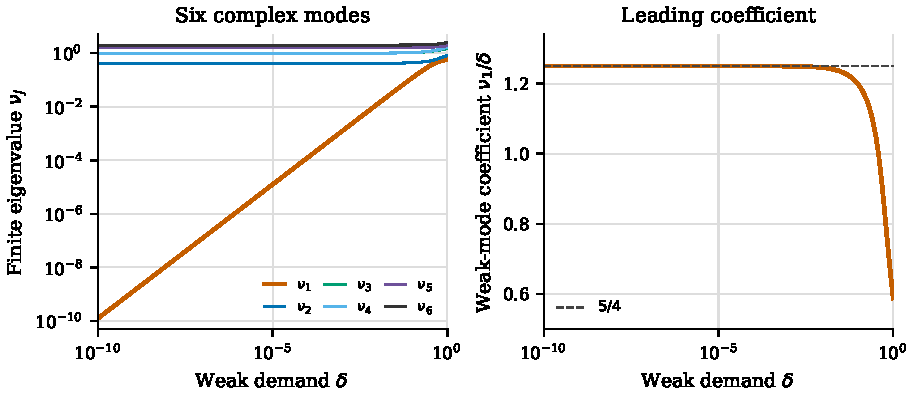
\includegraphics[width=\textwidth]{figures/output/weak_modes.pdf}
\caption{Finite commutator eigenvalues for demands $(\delta,1,1)$
(equivalently $t=1$ in the homogeneous finite model).
The first mode tends to zero while the other five stay positive;
the second panel displays its coefficient tending to $5/4$.
These are numerical evaluations of \eqref{eq:starform}, not
computed eigenvalues of the HE differential operator. Theorem~\ref{thm:star-scales}
supplies the relative comparison for small geometric $t$.}
\label{fig:weakmodes}
\end{figure}

\section{Scope and reproducibility}\label{sec:scope}

The theorem concerns a fixed compact Kähler background, fixed locally
free factors, two nonzero layers, and fixed multiplicities. Its
uniformity includes approaches to faces through the simple stable
region; it does not include the nonsimple endpoint itself. Higher
extensions have composable arrows and nonlinear integrability
relations, so the exact harmonic presentation and parity argument
used here do not apply without further work. Singular graded sheaves
and actual Yang--Mills flow estimates require additional analysis.

\subsection{Complex endomorphisms and adjoint symmetry}
Let $L_Z$ be the finite operator associated with
$\mathcal Q_{s,Z}$ and the rank mass. In orthonormal arrow
coordinates, direct expansion gives
\begin{equation}\label{eq:adjointsymmetry}
r_v\bigl((L_Z(X^*))_v-(L_ZX)_v^*\bigr)
=[X_v^*,\mu_s(Z)_v].
\end{equation}
At central balance the right side vanishes. Hence the Hermitian
real fixed space of adjoint complexifies to the full operator,
with the same eigenvalue multiplicities. This agrees with the
centralizer identity of~\cite[\S5.2, Proposition~5.3]{hkkp2023}.
Thus the six-mode example is a failure of scalar-vertex compression,
not a failure of correctly complexifying the Hermitian operator at
central balance.

Off balance a Hermitian restriction can lose even the correct
kernel. Take one target and one source, each of dimension two,
with arrows $I_2$ and
$J=\left(\begin{smallmatrix}0&1\\0&0\end{smallmatrix}\right)$.
The identity arrow forces the two centralizer blocks to agree;
commutation with $J$ then gives $X=Y=aI+bJ$. On the full
trace-free complex space the kernel is the line $X=Y=bJ$.
Its Hermitian part is zero. This representation is not centrally
balanced: its moments are $\operatorname{diag}(2,1)$ and
$\operatorname{diag}(-1,-2)$. It illustrates why the intermediate
gauge comparison in Lemma~\ref{lem:gaugespectrum} is performed
on the complex space. Likewise a single identity arrow has
connected support but all simultaneous matrix endomorphisms in
its centralizer. Connectedness alone never replaces the
scalar-centralizer condition.

\subsection{Finite calculations}
The accompanying scripts use the explicit matrices printed in
Section~\ref{sec:example}. Exact rational computations verify the
covariances, full centralizer dimension, positive trace-free Gram
form, characteristic polynomials, and the off-balance kernel
comparison above. A separate implementation forms the raw complex
commutator matrix in a Pauli basis and verifies the same six-mode
polynomial and the coefficient $25/20$. These calculations check
finite algebra; the proofs of HE existence and relative elliptic
estimates are those in Sections~\ref{sec:curvature}--\ref{sec:spectrum}.

For the plotted family we solve the two real target balance equations.
This is valid for these real matrices: uniqueness of the positive
Hermitian minimizer and invariance under complex conjugation imply
that it is real symmetric. Small eigenvalues are evaluated as the
squares of singular values of the commutator map restricted to a
mass-orthonormal trace-free basis. This avoids forming a rounded
Gram matrix before computing its weakest eigenvalue.
The numerical coefficient at $\delta=10^{-10}$ is approximately
$1.24999999996$, consistent with the proved limit $5/4$.

The source distribution contains the calculation scripts, generated
data, figure source, dependency versions, and commands for rebuilding
the figure and this PDF. No partial differential equation is solved
numerically in these computations. The numerical output is an
illustration and reproducibility check of the finite model, not an
additional hypothesis in the theorems.

\begin{thebibliography}{HKKP23}

\bibitem[CT24]{clarketipler2024}
A.~Clarke and C.~Tipler,
\emph{Semi-stability and local wall-crossing for Hermitian Yang--Mills connections},
J.\ Symplectic Geom.\ \textbf{22} (2024), no.~3, 673--694;
\href{https://arxiv.org/abs/2304.05245}{arXiv:2304.05245}.

\bibitem[Del25]{delloque2025}
R.~Delloque,
\emph{Continuity of HYM connections with respect to metric variations},
J.\ Lond.\ Math.\ Soc.\ (2) \textbf{112} (2025), no.~1, e70219;
\href{https://doi.org/10.1112/jlms.70219}{doi:10.1112/jlms.70219};
\href{https://arxiv.org/abs/2403.16814v4}{arXiv:2403.16814v4}.

\bibitem[HKKP23]{hkkp2023}
F.~Haiden, L.~Katzarkov, M.~Kontsevich, and P.~Pandit,
\emph{Semistability, modular lattices, and iterated logarithms},
J.\ Differential Geom.\ \textbf{123} (2023), no.~1, 21--66;
\href{https://doi.org/10.4310/jdg/1679503804}{doi:10.4310/jdg/1679503804};
\href{https://arxiv.org/abs/1706.01073v2}{arXiv:1706.01073v2}.

\bibitem[Kin94]{king1994}
A.~D.~King,
\emph{Moduli of representations of finite dimensional algebras},
Quart.\ J.\ Math.\ Oxford Ser.\ (2) \textbf{45} (1994), no.~4, 515--530;
\href{https://doi.org/10.1093/qmath/45.4.515}{doi:10.1093/qmath/45.4.515}.

\bibitem[Kob87]{kobayashi1987}
S.~Kobayashi,
\emph{Differential Geometry of Complex Vector Bundles},
Publications of the Mathematical Society of Japan \textbf{15},
Kan\=o Memorial Lectures \textbf{5}, Iwanami Shoten and Princeton
Univ.\ Press, 1987.

\bibitem[Lam26]{lam2026}
S.~T.~Lam,
\emph{Semistability and asymptotics of geometric flows},
preprint, 2026, \href{https://arxiv.org/abs/2606.09235v1}{arXiv:2606.09235v1}.

\bibitem[Wue26]{wuebben2026uniform}
B.~J.~Wuebben,
\emph{Uniform Hermitian--Einstein spectra for bipartite two-step extensions},
preprint, October 27, 2026,
\href{https://doi.org/10.5281/zenodo.23717123}{doi:10.5281/zenodo.23717123}.

\end{thebibliography}

\end{document}
